\documentclass{article}
\usepackage[english]{babel}
\usepackage[utf8]{inputenc}
\usepackage{a4wide}
\usepackage{booktabs}
\usepackage{xcolor}
\usepackage{fourier}
\usepackage[small,hang,bf]{caption}
\newcommand{\marcel}[1]{\footnote{Marcel: \color{red}#1}}
\usepackage{tabularx}
\usepackage{wrapfig}
\usepackage{setspace}
\usepackage[separate-uncertainty = true]{siunitx}
\usepackage{graphicx}
\usepackage{url}
\usepackage{pdfpages}
\definecolor{darkgreen}{rgb}{0,0.5,0}
\definecolor{darkblue}{rgb}{0,0,0.5}
\usepackage[colorlinks=true, urlcolor=darkblue, anchorcolor=darkblue, filecolor=green, linkcolor=darkblue, menucolor=darkblue,citecolor=darkblue,pdfpagemode=UseOutlines, pdfstartview=FitH,hypertexnames={false},bookmarksopen=true,breaklinks=true,pdfencoding=unicode]{hyperref}

\title{\LaTeX{} Quick Reference}
\author{Jaap Kokorian and Tjitte-Jelte Peters}


\begin{document}
\maketitle
\tableofcontents

\newpage
\section{Introduction}\label{sec:introduction}

This document offers some guidance to novice \LaTeX{} users. It is a list of frequently used \LaTeX{} commands and packages. With just the information in this document it is possible to create a manuscript that contains most commonly used typographic entities like bullets, enumerations, graphics, tables and math. Of course not all \LaTeX{} features are included in this list. But because \LaTeX{} has a very active online community, anything related to \LaTeX{} can be easily found by performing an online search.

\section{Commonly used \LaTeX~commands}

\begin{table}[htbp]
\caption{Document skeleton}
\begin{tabularx}{\textwidth}{lX}
	\toprule
	\LaTeX~command                                    & Description                                                                                     \\ 
	\midrule
	\verb|\documentclass|\verb|[<fontsize>,<paper>]{<type>}| & The start of every latex file. Sets the document class file to use.                             \\
	\verb|\usepackage|\verb|{}|                              & Loads a package.                                                                                \\
	\verb|\title|\verb|{<title>}|                            & Sets the document title.                                                                        \\
	\verb|\author|\verb|{<name>}|                            & Sets the author name or names.                                                                  \\
	\verb|\maketitle|                                 & Creates the title (article) or title page (report,book)                                         \\
	\verb|\tableofcontents|                           & Inserts a table of contents                                                                     \\
	\verb|\input|\verb|{file}|                               & Inserts the contents of \verb|file|.                                                            \\
	\verb|\include|\verb|{file}|                             & Inserts the contents of \verb|file| preceded and followed by a \verb|\clearpage|                \\
	\verb|\bibliographystyle|\verb|{stylefile}|              & Defines which .bst style file to use for the bibliography (use \verb|unsrt| if you don't care). \\
	\verb|\bibliography|\verb|{bibfile}|                  & Defines which .bib file to use and renders the bibliography section.                      \\ 
	\bottomrule
\end{tabularx}
\end{table}

\begin{table}[htbp]
\caption{Typeface changing commands}
\begin{tabularx}{\textwidth}{lX}
\toprule
\LaTeX~command & Description \\
\midrule
\verb|{\bf ..}| & bold font\\
\verb|{\it ..}| & italic font\\
\verb|{\ul ..}| & underlined font\\
\verb|\emph{..}| & emphasized font (usually italic, but may depend on document class)\\
\verb|$^\textnormal|\verb|{..}$| & Superscript \\
\verb|$_\textnormal|\verb|{..}$| & Subscript \\
\verb|{\small ..},{\normalsize ..},{\large ..} etc| & font size\\
\bottomrule
\end{tabularx}
\end{table}


\begin{table}[htbp]
\caption{Layout commands.}
\begin{tabularx}{\textwidth}{ll}
\toprule
\LaTeX~command & Description \\
\midrule
\verb|\newpage| & Pagebreak\\
\verb|\vspace|\verb|{..}| & Vertical space\\
\verb|\hspace|\verb|{..}| & Horizontal space\\
\verb|\\| & New line\\
\verb|<blank line>| & Paragraph break \\
\bottomrule
\end{tabularx}
\end{table}


\begin{table}[htbp]
\caption{Document structure}
\begin{tabularx}{\textwidth}{ll}
\toprule
\LaTeX~command & Hierarchy level \\
\midrule
\verb|\part|\verb|{..}| & -1\\
\verb|\chapter|\verb|{..}| & 0 (only books and reports)\\
\verb|\section|\verb|{..}| & 1\\
\verb|\subsection|\verb|{..}| & 2\\
\verb|\subsubsection|\verb|{..}| & 3\\
\verb|\paragraph|\verb|{..}| & 4\\
\verb|\subparagraph|\verb|{..}| & 5\\
\bottomrule
\end{tabularx}
\end{table}

\begin{table}[htbp]
\caption{References and citations}
\begin{tabularx}{\textwidth}{lX}
\toprule
\LaTeX~command & Description\\
\midrule
\verb|\label|\verb|{..}| & Inserts a label. Examples: \verb|\label|\verb|{fig:myFig}|, \verb|\label|\verb|{sec:theory}|, \verb|\label{eq:gauss}|.\\
\verb|\ref|\verb|{..}| & Inserts a reference to a label.\\
\verb|\eqref|\verb|{..}| & Inserts a reference to an equation (package \verb|amsmath|). Example: \verb|\eqref|\verb|{eq:gauss}|. \\
\verb|\cite|\verb|{..}| & Inserts a citation to a bibliographic item.\\
\verb|\pageref|\verb|{}| & Inserts a reference to the page number of a label.\\
\verb|\footnote|\verb|{..}| & Creates a superscript footnote symbol and puts the footnote text at the bottom of the page.\\
\bottomrule
\end{tabularx}
\end{table}

\newpage
\subsection{Dimensions}

Any time a command requires you to provide a length parameter (such as \verb|width|, \verb|height|, \verb|size|, etc.) you can enter a number with any of the following units: pt, cm, mm, in, px, ex, em and some more exotic ones. It is also possible to enter a fraction of a certain layout dimension such as: \verb|0.5\textwidth| or \verb|0.7\columnwidth|, which sets the dimension to half the text width or 0.7 times the column width (in case of multiple columns).


\newpage
\section{List structures}

\subsection{Enumeration}

\begin{minipage}[t]{0.5\textwidth}
{\LaTeX} command:
\vspace{3mm}

\verb|\begin{enumerate}|\\
\verb|\item| The first item\\
\verb|\item| The second item\\
\verb|\item| The last item\\
\verb|\end{enumerate}|
\end{minipage}
\begin{minipage}[t]{0.5\textwidth}
Result:
\begin{enumerate}
\item The first item
\item The second item
\item The last item
\end{enumerate}
\end{minipage}

\subsection{Itemization (bullet list)}

\begin{minipage}[t]{0.5\textwidth}
{\LaTeX} command:
\vspace{3mm}

\verb|\begin{itemize}|\\
\verb|\item| First\\
\verb|\item| Second\\
\verb|\item Third with subitems|\\
\verb|    \begin{itemize}|\\
\verb|    \item subitem|\\
\verb|    \item subitem|\\
\verb|    \end{itemize}|\\
\verb|\end{itemize}|\\
\end{minipage}
\begin{minipage}[t]{0.5\textwidth}
Result:

\begin{itemize}
\item First
\item Second
\item Third with subitems
	\begin{itemize}
	\item subitem
	\item subitem
	\end{itemize}
\end{itemize}
\end{minipage}

\section{Floating environments}

A floating environment is a document element of which the exact location cannot be directly controlled by the user, but is automatically determined by \LaTeX. Most floating environments have a 'caption': a block of text which is printed above or below the content.

All floating environments can be given an optional argument that specifies where \LaTeX{} should \emph{attempt} to place it. The options are \verb|h| (here), \verb|t| (top of the page), \verb|b| (bottom of the page) and \verb|p| (separate page). Multiple arguments can be given to specify in which order \LaTeX should attempt to place the floating environment. For example: \verb|[htbp]| means: try to place it here, if that fails place it on top of the page, on the bottom of the page, or, if that also fails, place it on it's own page. An exclamation mark behind one of the characters forces \LaTeX{} to try harder. The default float location argument is \verb|[tbp]|.

\subsection{Figure}

When rendered to PDF, \LaTeX{} supports the following image file formats: png, pdf, jpg.

\noindent\verb|\begin{figure}[htbp]|\\
\verb|\includegraphics{pics/something_interesting.pdf}|\\
\verb|\caption{This figure shows something interesting.}|\\
\verb|\label{fig:somethingInteresting}|\\
\verb|\end{figure}|

\newpage
\subsection{Table}

\begin{wraptable}[0]{r}{0.5\textwidth}
\centering
\caption{This is a table}
\begin{tabular}{rcl}
\toprule
A             & B     & C \\
\midrule
lorem         & ipsum & dolor \\
sit           & amet  & consectetur \\
adipisicing   & elit  & balls \\
\bottomrule
\end{tabular}
%\end{minipage}
\end{wraptable}
\begin{minipage}[t]{0.55\textwidth}
{\LaTeX} command:
\vspace{3mm}

\verb|\begin{table}[htbp]|\\
\verb|\centering|
\verb|\caption{This is a table}|\\
\verb|\begin{tabular}{rcl}|\\
\verb|\toprule|\\
\verb|A             & B     & C\\|\\
\verb|\midrule|\\
\verb|lorem         & ipsum & dolor \\|\\
\verb|sit           & amet  & consectetur \\|\\
\verb|adipisicing   & elit  & balls \\|\\
\verb|\bottomrule|\\
\verb|\end{tabular}|\\
\verb|\end{table}|\\
\end{minipage}
\begin{minipage}[t]{0.45\textwidth}
Result:
\end{minipage}

\section{Math}

\LaTeX{} is particularly good at typesetting mathematics. This section gives a brief overview of the possibilities. For a complete list of commands see: \url{http://en.wikibooks.org/wiki/LaTeX/Mathematics}.

\subsection{Inline math}

To type math expressions inside a normal paragraph, surround the math expression with dollar signs. Example: this sentence contains an inline formula that depends on $x$ and $y$. Here it is: $y=\int_{0}^{x} 2x'\textnormal{d}x'+3 $.


\subsection{Equation environment}

To place an equation on a separate line and let \LaTeX{} assign a reference number to it, use the equation environment:
\vspace{1em}

\noindent\verb|\begin{equation}|\\
\verb|\label{eq:NewtonsFirstLaw}|\\
\verb|F = m \cdot a|\\
\verb|\end{equation}|\\

\begin{equation}
\label{eq:NewtonsFirstLaw}
F = m \cdot a
\end{equation}

\newpage
\section{Essential packages}


\begin{itemize}
\item \verb|\usepackage[english]{babel}|: Ensures proper hyphenation in the English language.
\item \verb|\usepackage[utf8]{inputenc}|: Állöws typïng ôf ùníçøde chårâçtérs.
\item \verb|\usepackage[T1]{fontenc}|: extends the default OT1 7-bit font encoding of TeX to the T1 8-bit font encoding
\item \verb|\usepackage[small,bf,hang]{caption}|: Nicer captions for figures and tables.
\item \verb|\usepackage{xcolor}|: allows you to color text, like: \verb|{\color{red}{|..\verb|}| which will look {\color{red} like this}.
\item \verb|\usepackage{fourier}|: sets the font to Utopia which is nice and modern looking. Also provides lots of additional mathematics symbols.
\item \verb|\usepackage{booktabs}|: allows you to use the commands \verb|\toprule|, \verb|\midrule| and \verb|\bottomrule| in tables which is nice.
\item \verb|\usepackage{graphicx}|: without this package it is impossible to include figures!
\item \verb|\usepackage{amsmath}|: extended mathematics functionality
\item \verb|\usepackage{siunitx}|: typesetting numbers and units, see section \ref{sec:siunitx}.
\item \verb|\usepackage{hyperref}|: makes all citations, references and URLs \hyperref[clickable]{clickable} in the output pdf. \label{clickable}
\item \verb|\usepackage{cleveref}|: a cleverer way to do cross-referencing than the standard way. Import this package after all the others.
\end{itemize}


\subsection{SIunitx}\label{sec:siunitx}

The \verb|siunitx| package introduces a set of absolutely essential commands for typesetting numbers with units. Never again look for the `mu' symbol, but simply type \verb|\SI{10}{\micro\metre}|, to get \SI{10}{\micro\metre}. Note that the space between the number and the unit is slightly smaller than the space between two words, which is exactly the way it is supposed to be and which is really tedious to accomplish with a program like MS Word.

Also the readability of large numbers like `1000000' can be improved by writing \verb|\num{1000000}|, which results in \num{1000000}. Delimiters (thin spaces in this case) divide the number in groups consisting of no more than three digits.

\begin{wraptable}[8]{r}{0.4\textwidth}
\caption{A table with aligned numbers}
\centering
\begin{tabular}{S S[table-parse-only]}
\toprule
{Decimal-centered} &
{Regular centering} \\
\midrule
1234.5 & 1234.5 \\
-88.8(9) & -88.8(9) \\
4.5e+5 & 4.5e5 \\
\bottomrule
\end{tabular}
\label{tab:someTable}
\end{wraptable}

Finally, \verb|siunitx| supports automatic alignment of the numbers within table columns. This enables for example centering on the decimal marks. All you need to do is change the column argument of the tabular command. Example: \verb|\begin{tabular}{S S[table-parse-only]}|. This example will result in a table with two columns. The left column will be decimal-centered while the right column will be centered in the regular way.

\clearpage
\section{Optional packages}
The packages listed here are not required to create a document, but provide functionality you might desire occasionally.

\begin{itemize}
\item \verb|\usepackage{fullpage}|: Uses the entire page for the document.
\item \verb|\usepackage{geometry}|: Allows you to manually specify the dimensions of margins, headers, footers, etc.
\item \verb|\usepackage{todonotes}:| Allows you to add little todo notes in the document and its margins, insert missing figure placeholders and print a list of all todos.
\item \verb|\usepackage{natbib}|: Extended literature citation functionality.
\item \verb|\usepackage{glossaries}|: To create glossaries, nomenclatures and alike.
\end{itemize}


\appendix

\section{LaTeX typesetting style guide}

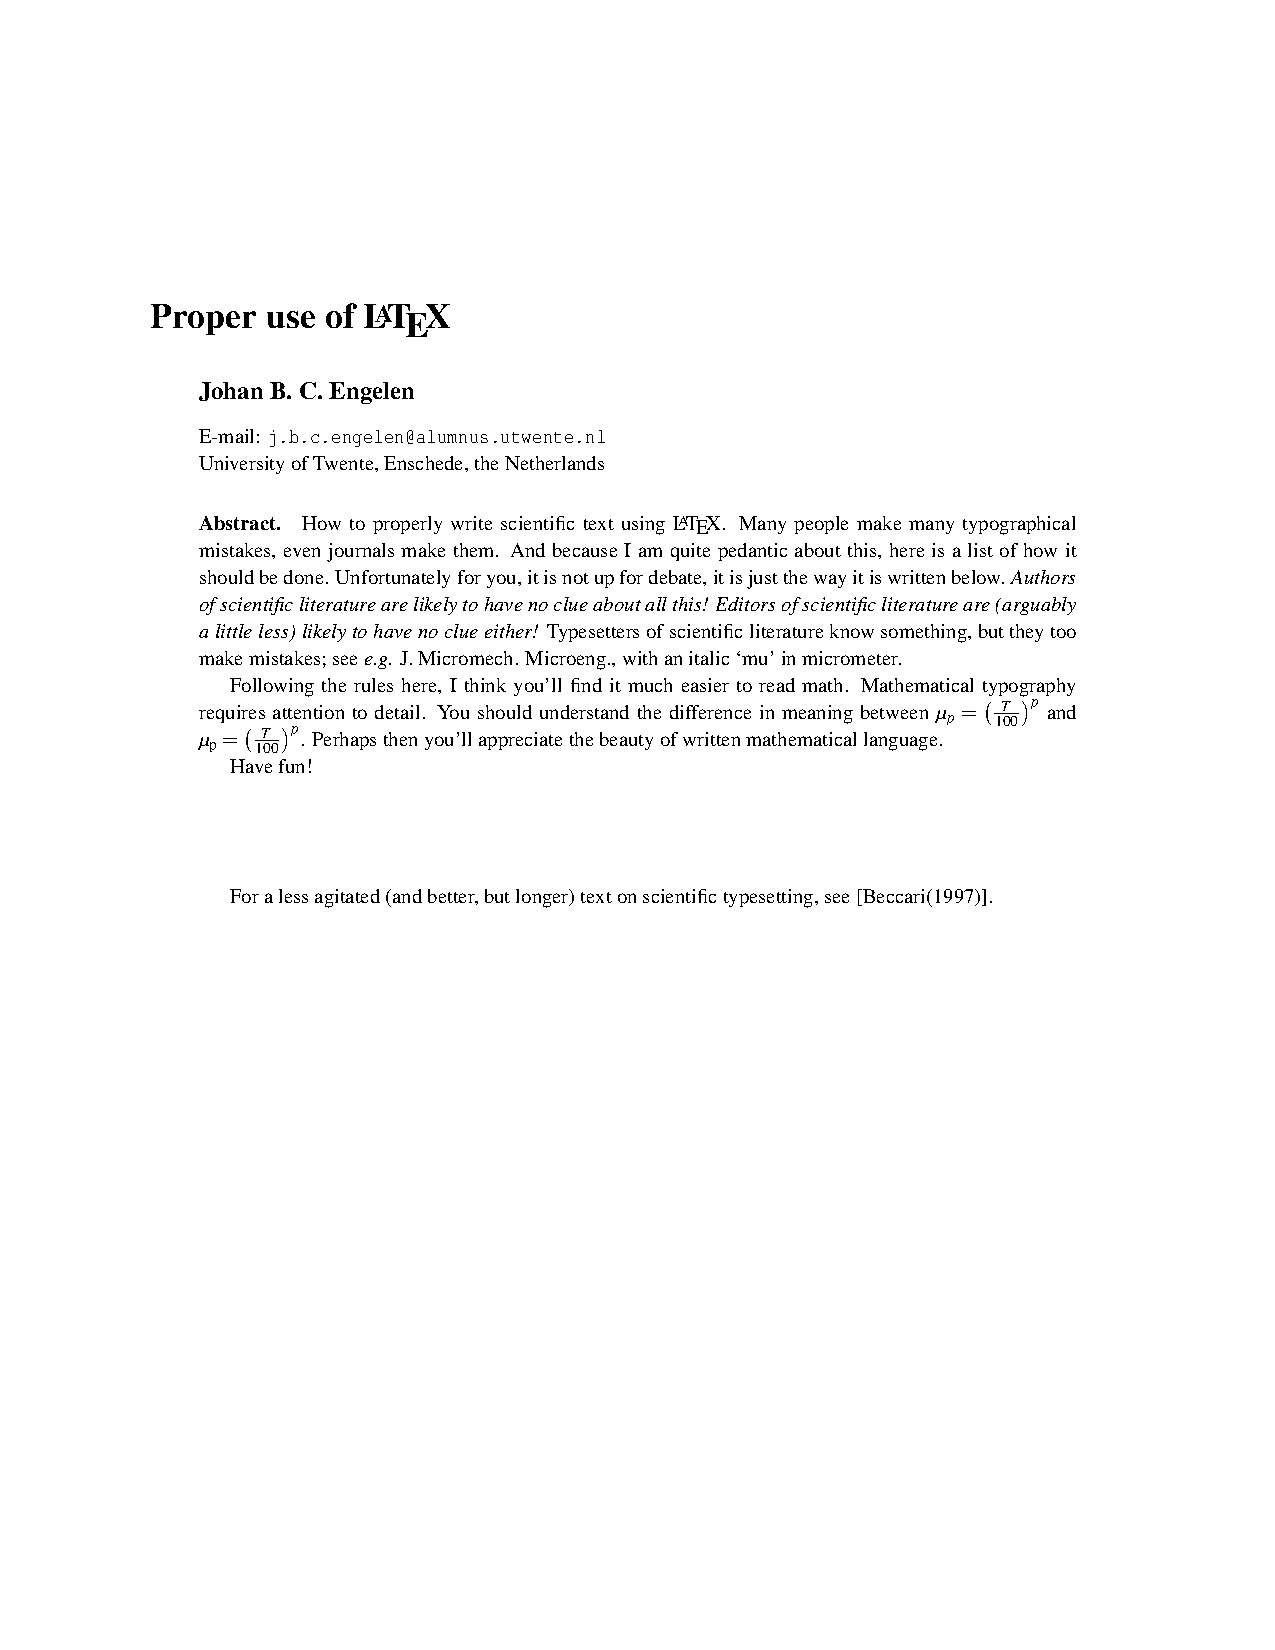
\includepdf[pages=-]{ProperUseOfLaTeX}

\end{document}